\documentclass{standalone}
\usepackage{pgfplots}
\pgfplotsset{compat=1.7}

\begin{document}
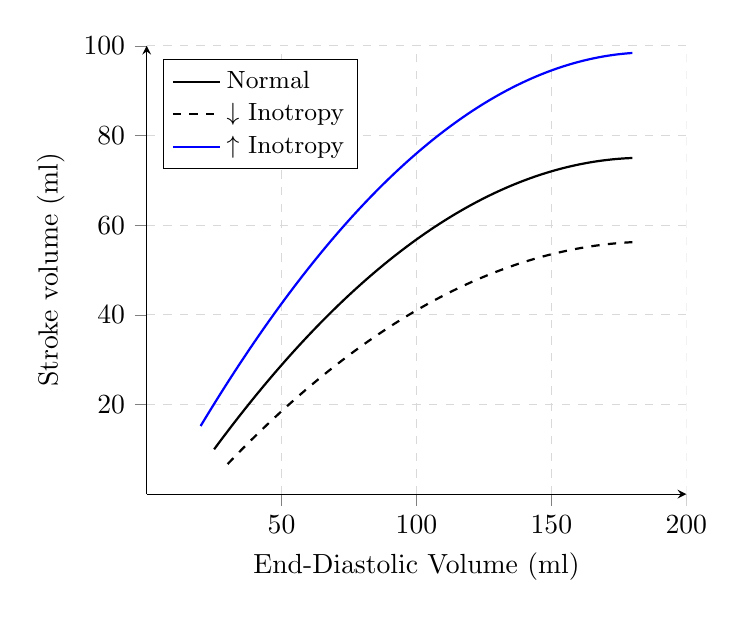
\begin{tikzpicture}


\begin{axis}[
        axis lines=middle,
        grid = major,
        grid style={dashed, gray!30},
	ymin = 0,
	ymax = 100,
	xmin = 0,
xmax =200,
        grid = major,
	 ylabel near ticks,
	xlabel near ticks,
        xlabel=End-Diastolic Volume (ml),
        ylabel=Stroke volume (ml),
        tick align=outside,
        enlargelimits=false,
legend pos= north west,
legend style={font=\small, cells={align=left}},
legend cell align={left}]

\plot[domain=25:180, black, thick,samples=500] {-12 + 0.944*x - 0.00256*x^2};
\addlegendentry{Normal}
\plot[domain=30:180, black, dashed, thick,samples=500] {-14 + 0.75*x - 0.002*x^2};
\addlegendentry{$\downarrow$ Inotropy}
\plot[domain=20:180, blue, thick,samples=500] {-6 + 1.12*x - 0.003*x^2};
\addlegendentry{$\uparrow$ Inotropy}


\end{axis}

\end{tikzpicture} 
\end{document}